\section{Incrementally compute matrix programs}
Matrix operations are quite ubiquitous in modern data analysis tasks, which usually involve small incremental data analysis where the datasets are dynamic. To effectively propagate the input changes through the matrix operation program to the output, there are some efforts which consider matrix as views and accomplish the goal of incremental view maintenance. One example is Linview \cite{nikolic2014linview}, which targets at converting iterative programs with basic matrix manipulation primitives: matrix addition, multiplication, subtraction, transpose and inverse, into a {\em trigger program} and propagating the {\em delta expressions} via the trigger programs to derive the new output rather than re-evaluating from the scratch. In what follows, how the authors of \cite{nikolic2014linview} model the iterative programs with matrix operations, represent and propagate {\em delta expressions} and deal with typical linear algebra programs are elaborated respectively.

\subsection{Model the iterative programs}\label{sec: iterative_model}
Iterative computation is very common in data analysis programs, for which naive re-evaluation from the scratch in the case of data updates can incur high over head. Under the assumption that the iterative programs end after a fixed number of iteration steps (even after updates), Linview deals with delta expression propagation through the program under three different iterative models.

\paragraph{Linear model} The first iterative model is {\em linear model}, which simply updates the result at $k_{th}$ epoch based on the results at $(k-1)_{th}$ epoch. Given the input $A$, the output at epoch $k$ is computed as:

\[T_k=
\begin{cases}
f(A)& k=1\\
g(T_{k-1}, A) & k=2,3,\dots\\
\end{cases}
\]

\paragraph{Exponential model} In the {\em exponential model}, the output at $k_{th}$ epoch depends on the result at $(k/2)_{th}$ epoch, which has larger steps compared to {\em linear model}, i.e.:

\[
T_k=
\begin{cases}
f(A)& k=1\\
g(T_{k/2}, A) & k=2,4,8\dots\\
\end{cases}
\]

\paragraph{Skip model} {\em Skip model} lies in between, in which the step between the computed iterations is adjustable. Given a skip size $s$, the result before $s_{th}$ epoch is computed by {\em exponential model} and then the result after $s_{th}$ epoch is computed every $s_{th}$ iteration. The {\em skip model} is thus represented as:

\[
T_k=
\begin{cases}
f(A)& k=1\\
g(T_{k/2}, A) & k=2,4,8\dots,s\\
h(T_{k-s}, T_{s}, A) & k=s, 2s,\dots
\end{cases}
\]

\subsection{Incremental computation}
This subsection is centered around how Linview represent and propagate delta computation through the linear algebra program, which starts by introducing the incremental updates over matrix manipulation primitives. Matrix multiplications are frequently used in the following analysis, which is assumed to have time complexity $O(n^{\gamma})$ ($2\leq \gamma \leq 3$, varies for different algorithms)

\paragraph{Delta rules for basic matrix operations}
Given a matrix $A$ and a function $f(*)$, small changes $\Delta A$ to $A$ leads to the changes of output of $f(A)$ as: $\Delta_A(f) = f(A+\Delta A) - f(A)$. By following the properties of basic matrix operations, such as matrix addition, matrix multiplication and matrix inverse, the delta rule is shown as follows:

\begin{center}
    \begin{minipage}{0.4\textwidth}
      \begin{itemize}
        \item $\Delta_A(f_1 f_2) = f_2\Delta_A(f_1) + f_1\Delta_A(f_2)$
        \item $\Delta_A(f_1 \pm f_2) = \Delta_A(f_1) \pm \Delta_A(f_2)$
        \item $\Delta_A(\lambda f) = \lambda \Delta_A(f)$
        \item $\Delta_A(f^{-1}) = f(A+\Delta A)^{-1}-f(A)^{-1}$
      \end{itemize}
    \end{minipage}
  \end{center}

Note that for most update rules shown above, the time complexity is $O(n^2)$ while in general case, the delta derivation for matrix inverse has the same overhead as reevaluation from the scratch, which is much more expensive than $O(n^2)$. However, under the assumption that $\Delta A$ is relatively small than $A$ and thus have lower rank ($k$) than $A$ ($n$) where $k \ll n$, $\Delta A$ can be decomposed into multiplication of vectors and thus much cheaper for computation, which is called {\em factored form}. For example, given a rank-1 $\Delta A$ ($=\bar{u}\bar{v}^T$), by applying Sherman-Morrison formula \cite{press2007numerical}, $\Delta_A(\lambda f)$ can be written as:

\begin{equation}\label{eq: matrix_inverse}
\Delta_A(f^{-1}) = -\frac{f(A)^{-1}\bar{u}\bar{v}^Tf(A)^{-1}}{1+\bar{v}^Tf(A)^{-1}\bar{u}}
\end{equation}

\paragraph{Delta representation}
The overhead of incremental updates also relies on how to represent the delta. It has turned out that naive representations won't help even for very simple program with very minor changes. 

\begin{example}\label{eg: incremental_naive_update}
For example, consider the following program to compute $A^8$ for an $n\times n$ matrix $A$:

\begin{center}
    $B:= AA$\\
    $C:= BB$\\
    $D:= CC$
\end{center}

Given a small change $\Delta A$, such as an update to the entry $A_{i,j}$, $\Delta A_{i,j}$, which has overhead $O(1)$, by applying the delta rules for matrix multiplication mentioned above, $\Delta B$, $\Delta C$ and $\Delta D$ are represented as:

\begin{equation}\label{eq: delta_b}
    \Delta B = (\Delta A) A + A (\Delta A) + (\Delta A) (\Delta A)
\end{equation}
\begin{equation}\label{eq: delta_c}
    \Delta C = (\Delta B) B + B (\Delta B) + (\Delta B) (\Delta B)
\end{equation}
\begin{equation}\label{eq: delta_d}
    \Delta D = (\Delta C) C + C (\Delta C) + (\Delta C) (\Delta C)
\end{equation}
    


Computing $\Delta B$ only requires $O(n)$ operations since $(\Delta A) A$ and $A (\Delta A)$ only need to scale the $i_{th}$ row and $j_{th}$ column of $A$ by $\Delta A_{i,j}$ respectively, which takes $O(n)$ time while $(\Delta A) (\Delta A)$ only incurs $O(1)$ overhead. In the end, compared to original $B$, the changes caused by $\Delta B$ appear in the $i_{th}$ row and $j_{th}$ column of $B$.

Similarly, we can derive that $\Delta C$ requires $O(n^2)$ operations, which ends up with the full updates to the entire $C$. The effect of update propagation is shown in Figure \ref{fig:update_propagete}.

\begin{figure}
    \centering
    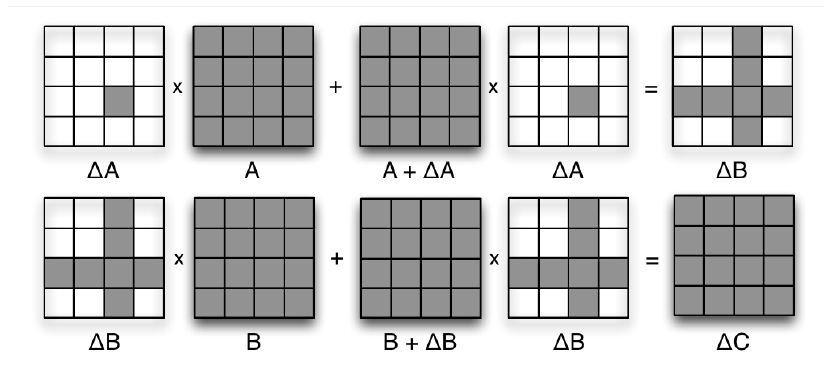
\includegraphics[width=10cm, height=4cm]{Figures/update_propagation.png}
    \caption{The effect of updates propagate}
    \label{fig:update_propagete}
\end{figure}

Then computing $\Delta D$ involves at least two full $O(n^{\gamma})$ matrix multiplications, which is obviously more expensive than recomputing $\Delta D$ from the scratch. \qed
\end{example}


To deal with this unexpected effect, the delta expressions are all represented as Example \ref{eg: incremental_naive_update} indicates, the updates $\Delta A$ is only a change to a single entry $A_{i,j}$, which is a rank-1 update and can be represented as $\Delta A = \bar{u}\bar{v}^T$ where $\bar{u}$ and $\bar{v}$ are both column vectors. Then by replacing $\Delta A$ in Equation \ref{eq: delta_b} with $\bar{u}\bar{v}^T$, $\Delta B$ is rewritten as:
\begin{equation}\label{eq: update_b_product}
\Delta B = \bar{u}(\bar{v}^TA) + (A\bar{u})\bar{v}^T + (\bar{u}\bar{v}^T\bar{u})\bar{v}^T=[\bar{u}, (A\bar{u}), (\bar{u}\bar{v}^T\bar{u})]
\begin{bmatrix}
    (\bar{v}^TA)  \\
    \bar{v}^T  \\
    \bar{v}^T   
\end{bmatrix}
=[\bar{u}_1, \bar{u}_2, \bar{u}_3]
\begin{bmatrix}
    \bar{v}^T_1  \\
    \bar{v}^T_2  \\
    \bar{v}^T_3  
\end{bmatrix}
\end{equation}

which is a sum of three outer products. The term $(\bar{v}^TA)$, $(A\bar{u})$ and $(\bar{u}\bar{v}^T\bar{u})$ can be all derived in $O(n^2)$ time while the vector $[\bar{u}, (A\bar{u}), (\bar{u}\bar{v}^T\bar{u})]$ and $[(A^T\bar{v}), \bar{v}, \bar{v}]$ are both $n \times 3$ matrices and thus the product of them requires $O(3n^2)$ operations.

In general, all the delta expressions can be expressed as a product of two $n \times k$ matrices where $k \ll n$, which only requires $O(kn^2)$ operations, although it is more expensive than naive updates for $\Delta B$ as shown in Example \ref{eg: incremental_naive_update}. For example, for $\Delta C$, since it is a sum of three products and each of them can be expressed as a product of two $n \times 3$ matrices by inserting Equation \ref{eq: update_b_product} to Equation \ref{eq: delta_c}, $\Delta C$ can thus be expressed as a a product of two $n \times 9$ matrices:


\begin{equation}
\begin{split}
    \Delta C &= (\Delta B) B + B (\Delta B) + (\Delta B) (\Delta B) \\&=[\bar{u}_1, \bar{u}_2, \bar{u}_3]
\begin{bmatrix}
    \bar{v}^T_1B \\
    \bar{v}^T_2B \\
    \bar{v}^T_3B 
\end{bmatrix}+[B\bar{u}_1, B\bar{u}_2, B\bar{u}_3]
\begin{bmatrix}
    \bar{v}^T_1 \\
    \bar{v}^T_2 \\
    \bar{v}^T_3 
\end{bmatrix}\\
&+[\bar{u}_1, \bar{u}_2, \bar{u}_3]
\begin{bmatrix}
    \bar{v}^T_1  \\
    \bar{v}^T_2  \\
    \bar{v}^T_3  
\end{bmatrix}
[\bar{u}_1, \bar{u}_2, \bar{u}_3]
\begin{bmatrix}
    \bar{v}^T_1  \\
    \bar{v}^T_2  \\
    \bar{v}^T_3  
\end{bmatrix}\\
&=[\bar{u}_1, \bar{u}_2, \bar{u}_3, B\bar{u}_1, B\bar{u}_2, B\bar{u}_3, \bar{u}_1, \bar{u}_2, \bar{u}_3]\\
&\begin{bmatrix}
    \bar{v}^T_1B \\
    \bar{v}^T_2B \\
    \bar{v}^T_3B \\
    \bar{v}^T_1  \\
    \bar{v}^T_2  \\
    \bar{v}^T_3  \\
    \bar{v}^T_1(\bar{u}_1\bar{v}^T_1 + \bar{u}_2\bar{v}^T_2 + \bar{u}_3\bar{v}^T_3)\\
    \bar{v}^T_2(\bar{u}_1\bar{v}^T_1 + \bar{u}_2\bar{v}^T_2 + \bar{u}_3\bar{v}^T_3)
    \bar{v}^T_3(\bar{u}_1\bar{v}^T_1 + \bar{u}_2\bar{v}^T_2 + \bar{u}_3\bar{v}^T_3)
\end{bmatrix}
\end{split}
\end{equation}

which requires $O(9n^2)$ operations in total. Finally, by inserting the expression of $\Delta C$ above into Equation \ref{eq: delta_d}, computing $D$ only requires $O(27n^2)$ operations, which is far cheaper than re-evaluation from the scratch.

Actually, $\Delta B$ can be further optimized as:
\begin{equation}\label{eq: update_b_product_opt}
\Delta B = \bar{u}(\bar{v}^TA) + (A\bar{u})\bar{v}^T + (\bar{u}\bar{v}^T\bar{u})\bar{v}^T=[\bar{u}, (A\bar{u}) + (\bar{u}\bar{v}^T\bar{u})]
\begin{bmatrix}
    (\bar{v}^TA)  \\
    \bar{v}^T 
\end{bmatrix}
=[\bar{u}_1', \bar{u}_2']
\begin{bmatrix}
    \bar{v}^T_1'  \\
    \bar{v}^T_2'  \\
\end{bmatrix}
\end{equation}

which is a product of two $n \times 2$ matrices. Consequently, $\Delta C$ and $\Delta D$ can be represented as a product of two $n \times 4$ matrices and two $n \times 8$ matrices respectively.

\paragraph{Constructing trigger functions}
Given the derivation rules above, Linview converts the linear algebra program into a set of trigger functions, which takes a set of input matrices and handle the updates of them sequentially. For example, given a set of input matrices $D=\{A, B, \dots\}$ and an evaluation function $f(*)$ over that, then the overall effect of updates will to $f(D)$ will be:

\begin{equation}\label{eq: updates_by_multi_vars}
\Delta_{D}(f(D)) = \Delta_{A}(f(D)) + \Delta_{D\\\{A\}}(f(D) + \Delta_{A}(f(D)))
\end{equation}


%  and Linview generates one trigger function for each of them, which is then used to monitor the change of the corresponding input matrix.

\subsection{Incremental analysis for typical programs}
The incremental update model above can fit some typical linear algebra programs, such as ordinary least squares, matrix powers and even more general forms, which are illustrated below.

\paragraph{Ordinary least squares}
Ordinary least squares is a classic regression problem, for which we need to derive the best parameter $\beta^*$ for a linear system, $Y = X\beta$ ($X$ is a $m \times n$ matrix representing predictors while $Y$ is a $m \times p$ matrix for response variables) through statistical estimates. With some typical statistic assumptions, such as Gaussian noise, the best estimates for $\theta$ is $\theta^* = (X^TX)^{-1}X^TY$.

In practice, the regression model is usually built in a dynamic environment where the incoming new data requires efficient model updates on the basis of the outdated model instead of computing from the scratch every time, for which the performance bottleneck is to update the inverse operation $(X^TX)^{-1}$. We represent $X^TX$ as $Z$. So given a rank-1 update to $X$, i.e. $\Delta X = \bar{u}\bar{v}^T$, $\Delta Z$ can be expressed as:
\begin{equation}
    \Delta Z = [\bar{v}\ \ (X^T\bar{u} + \bar{v}\bar{u}^T\bar{u})]\begin{bmatrix}
    \bar{u}^T X  \\
    \bar{v}^T  
\end{bmatrix}\\
=[\bar{p}_1\ \bar{p}_2]\begin{bmatrix}
    \bar{q}^T_1  \\
    \bar{q}^T_2  
\end{bmatrix}=\bar{p}_1\bar{q}_1^T + \bar{p}_2\bar{q}_2^T
\end{equation}

It has time complexity $O(mn)$ due to the computation of $X^T\bar{u}$, $\bar{v}\bar{u}^T\bar{u}$ and $\bar{u}^TX$, which ends up with a product of two $n\times 2$ matrices and thus a rank-2 update to $Z$. We can further $\Delta Z_1 = \bar{p}_1\bar{q}_1^T$ and $\Delta Z_2 = \bar{p}_2\bar{q}_2^T$ such that $\Delta Z_1$ and $\Delta Z_2$ are both rank-1 matrix. Considering the fact that both $X$ and $\Delta X$ are $m \times n$ matrices and thus $\bar{u}$ and $\bar{v}$ are $m \times 1$ and $n \times 1$ vector respectively, $\bar{p}_1$ and $\bar{q}_2$ should be both $n \times 1$ vectors. Besides, the computation result of $X^T\bar{u}$ and $\bar{v}\bar{u}^T\bar{u}$ are both $n \times 1$ vector and thus $\bar{p}_2$ (sum of $X^T\bar{u}$ and $\bar{v}\bar{u}^T\bar{u}$) should be also $n \times 1$ vector. Similarly, $\bar{q_1}^T$ is also $n \times 1$ vector.

By following Equation \ref{eq: matrix_inverse} and Equation \ref{eq: updates_by_multi_vars}, the update rules for $W = (X^TX)^{-1} = Z^{-1}$ with respect to $\Delta Z_1$ and $\Delta Z_2$ will be:

\begin{center}
\begin{equation}
\begin{split}
    \Delta_{Z_1}(W)& = -\frac{W\bar{p}_1\bar{q}_1^TW}{1 + \bar{q}_1^TW\bar{p}_1}\\
    \Delta_{Z_2}(W)& = -\frac{(W+\Delta_{Z_1}(W))\bar{p}_2\bar{q}_2^T(W+\Delta_{Z_1}(W))}{1 + \bar{q}_2^T(W+\Delta_{Z_1}(W))\bar{p}_2}
\end{split}   
\end{equation}
\end{center}

while simply computes the rank-1 update $\Delta Z_1$ to $W$ and then accumulate the effect of $\Delta Z_2$ for $W$. $\Delta_{Z_1}$ and $\Delta_{Z_2}$ can be further written as:

\begin{equation}
\begin{split}
\Delta_{Z_1}(W) = \bar{r}_1\bar{s}_1^T\\    
\Delta_{Z_2}(W) = \bar{r}_2\bar{s}_2^T
\end{split}
\end{equation}

where $\bar{r}_1 = W\bar{p}_1$, $\bar{r}_2 = (W+\Delta_{Z_1}(W))\bar{p}_2$ while $\bar{s}_1$ and $\bar{s}_2$ are the rest of the subexpressions of $\Delta_{Z_1}(W)$ and $\Delta_{Z_2}(W)$ respectively. So the overall updates to $W$ is $\Delta W = \bar{r}_1\bar{s}_1^T + \bar{r}_2\bar{s}_2^T$, which is a rank-2 update.
Since $\bar{p}_i$ and $\bar{q}_i$ ($i=1,2$) are column vector of length $n$ and $Z$ and $W$ are $n \times n$ matrices, the computation of $\bar{r}_1 = W\bar{p}_1$ thus need $O(n^2)$ operations, which is the same for $\bar{s}_1$, $\bar{s}_2$ and $\bar{r}_2$. So the overall cost to update $W$ is thus $O(n^2 + mn)$, which is far less than the cost of recomputing from the scratch, i.e. $O(n^3 + mn)$.

In terms of the update for $\beta^*$ (denoted by $\Delta \beta$), given the update to the input $X$, i.e. $\Delta X=\bar{u}\bar{v}^T$, $\Delta \beta$ can be thus written as:

\begin{equation}
    \Delta \beta = \Delta WX^TY + W\Delta X^TY + \Delta W\Delta X^TY = (\bar{r}_1\bar{s}_1^T + \bar{r}_2\bar{s}_2^T)X^TY + W\bar{v}\bar{u}^TY + (\bar{r}_1\bar{s}_1^T + \bar{r}_2\bar{s}_2^T)\bar{v}\bar{u}^TY
\end{equation}

while requires $O(n^2 + mp + np + mn)$ operations in total while re-evaluation incurs $O(mnp + n^2min(m,p))$ operations.

\paragraph{Matrix powers}
The goal of matrix powers is to compute $A^k$ for an input matrix $A$ with a given exponent $k$, which plays an important role in many data analysis tasks. Matrix powers can be computed iteratively, for which the three iterative models proposed in \ref{sec: iterative_model} is applicable and the trade-offs between the three models can be explored under re-evaluation strategy or incremental update strategy.

The time and space complexity of matrix powers under different iterative models and different evaluation strategies (re-evaluation or incremental update) is presented in Figure \ref{fig:time_space_complexity_matrix_power}. Under the assumption that $k \ll n$ 

\begin{figure}
    \centering
    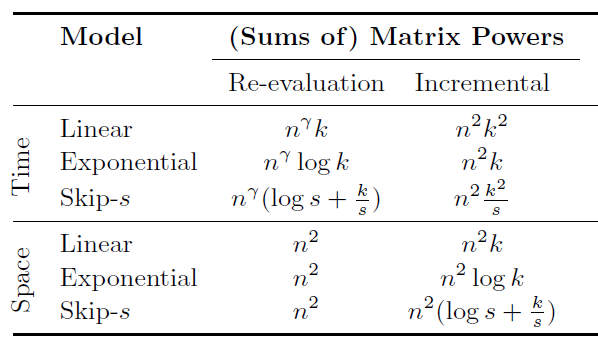
\includegraphics[width=8cm, height=4.5cm]{Figures/time_space_complexity_matrix_powers.png}
    \caption{The time and space trade-offs for matrix power}
    \label{fig:time_space_complexity_matrix_power}
\end{figure}

For re-evaluation strategy, it would require $O(n^{\gamma})$ operations for every iteration and thus the total time complexity depends on the number of iterations. Thus Exponential model outperform other models since it has largest leap between iterations. But all of the models have the same space complexity, i.e. $O(n^2)$.

For incremental update strategy, the computation time at each iteration should be $O(rn^2)$ where $r$ is the rank of the input delta expression on the updates at each iteration and the rank of delta expression increases linearly as the iteration proceed, which leads to the nearly quadratic running time and linear space consumption with respect to iteration number.

Similar to {\em matrix power}, the sum of matrix power problem, which aims at computing $S_k = I + A + A^2 + \dots + A^k$ given input $A$ and maximum exponent $k$ where $I$ is the identity matrix, have the almost the same computation process and thus have the same time complexity as shown in Figure \ref{fig:time_space_complexity_matrix_power}. 

\paragraph{General form} The authors also consider a general iterative matrix computation programs based on matrix powers, i.e. $T_{i+1} = AT_{i} + B$ where $A$ is the input matrix with dimension $n \times n$, $B$ is a constant matrix with dimension $n \times p$ and the result of $T_{i}$ is iteratively computed with dimension $n \times p$. Such general form appears in many applications such as PageRank and power iteration method for eigenvalue computation. 

Note that $T_{i+1} = AT_{i} + B$ can be unrolled as the form for computing $T_{i+k}$, i.e. $T_{i+k} = A^kT_{i} + (A^{k-1} + A^{k-2} + \dots + A + I) B$, in which how to efficiently incrementally compute $P_k = A^k$ and $S_k = (A^{k-1} + A^{k-2} + \dots + A + I)$ has been discussed before and thus both $P_k$ and $S_k$ are materialized and maintained along with $T_k$. Given those notations, the derivation rules for $T_{i+1} = AT_{i} + B$ under the three iterative models from Section \ref{sec: iterative_model} are shown in Table \ref{tab:derivation_rule}.

\begin{table}[]
    \centering
    \begin{tabular}{|c|c|}\hline
        Model & Derivation rule \\ \hline
        Linear & $T_k=
\begin{cases}
AT_0 + B& k=1\\
AT_{i-1} + B & k=2,3,4\dots,k
\end{cases}$\\ \hline
        Exponential & $T_k=
\begin{cases}
AT_0 + B& k=1\\
P_{i/2}T_{i/2} + S_{i/2}B & k=2,4,8\dots,s\\
\end{cases}$\\ \hline
        Skip-s &$T_k=
\begin{cases}
AT_0 + B& k=1\\
P_{i/2}T_{i/2} + S_{i/2}B & k=2,4,8\dots,s\\
P_sT_{i-s} + S_sB & k = 2s, 3s, \dots, k
\end{cases}$\\ \hline
    \end{tabular}
    \caption{Derivation rules for $T_{i+1} = AT_{i} + B$ under three iterative models}
    \label{tab:derivation_rule}
\end{table}

Then given an update $\Delta A$ against the input matrix $A$, the cost analysis under different iterative models and update strategies is provided below.

In terms of re-evaluation strategy, the results of $T_i$, $P_i$ and $S_i$ are only materialized for current iteration. For linear model, computing $AT_i$ is the performance bottleneck, which requires $O(np)$ operations (the result has dimension $n \times p$) with $O(n)$ multiplications for each operation. So the total time complexity is $O(pn^2)$ for each iteration and thus $O(pn^2)$ for $k$ iterations. For exponential model and skip-s model, maintaining $P_i$ and $S_i$ would incur time complexity $O(n^{\gamma})$ for every iterations, which is essential for $logk$ and $logs$ iterations respectively. Besides the cost of maintaining the auxiliary matrices $P_i$ and $S_i$, it still needs $O(pn^2)$ time to compute $P_sT_{i-s}$ or $P_{i/2}T_{i/2}$ at each iteration. Since the number of iterations for exponential model and skip-s model is $logk$ and $logs + \frac{k}{s}$ respectively, the overall time complexity for the two models will be $O(n^{\gamma} + pn^2)logk$ and $O(n^{\gamma}logs + pn^2(logs+ \frac{k}{s}))$.

For incremental strategy, the time complexity to maintain $P_s$ and $S_s$ is still $O(n^2)$ for each iteration as discussed before. To derive $T_k$, the update rule $P_{i/2}T_{i/2} + S_{i/2}B$ or $P_sT_{i-s} + S_sB$ is used, which requires extra $O(np)$ time to compute the factored form for $T_i$. So the overall time complexity for each iteration will be $O(n^2 + np)$. By following similar analysis for {\em matrix powers}, the time complexity and space complexity for the three different iterative models is presented in Figure \ref{fig:time_space_complexity_general_form}.

But notice that for some extreme case, such as $p=1$, incremental update strategy has worse performance than re-evaluation strategy, which is due to the unnecessary factor form representations for $T_i$ (a vector in this case). To solve this problem, a combination of the re-evaluation strategy and incremental updates strategy is proposed, which simply represent delta expression for $T_i$ as a single matrix instead of two factored vectors and still represent the auxiliary matrix $P_i$ and $S_i$ in factored form. So for exponential model and skip-s model, they require $rn^2$ operations to update $P_i$ and $S_i$ for each iteration where $r$ is the rank of them, which incurs the same overhead as the incremental updates for matrix powers while the time complexity to compute $T_k$ is $O(pn^2)$ when $P_i$ and $S_i$ are given, which has the same time complexity as re-evaluation strategy. By summing up the time complexity from the two parts, the overall time complexity is presented in Figure \ref{fig:time_space_complexity_general_form}. Since both $P_i$ and $S_i$ for hybrid strategy are materialized in the same form as incremental update strategy for every iteration, it thus shares the same space complexity as incremental update strategy.


\begin{figure}
    \centering
    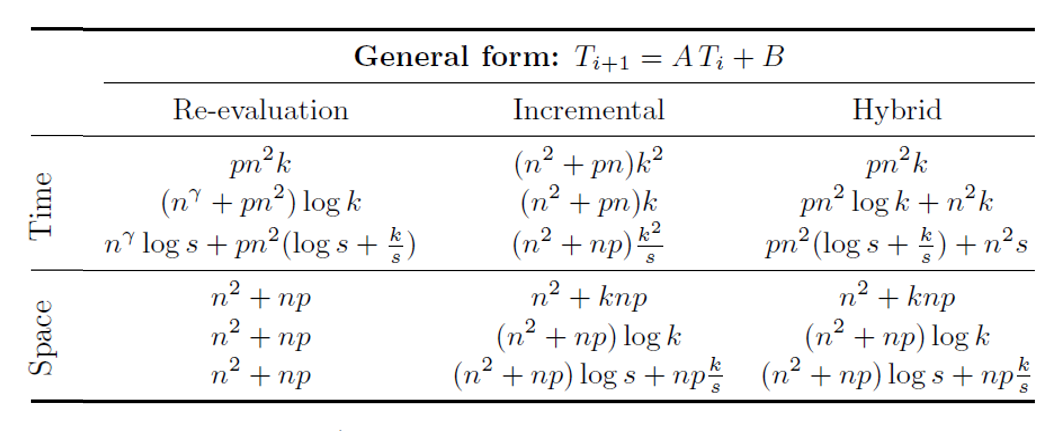
\includegraphics[width=12cm, height=4.5cm]{Figures/time_space_complexity_general_form.png}
    \caption{The time and space trade-offs for general forms}
    \label{fig:time_space_complexity_general_form}
\end{figure}


\subsection{Discussions}
